\documentclass[11pt,a4paper]{article}
% Presumably we will have a modified template header for the final papers
% For now we hard code things below

\usepackage{fancyhdr}
\usepackage{parskip}
\usepackage[usenames,dvipsnames]{color}
\usepackage[colorlinks=true, linkcolor=BrickRed, citecolor=Blue, urlcolor=Blue, filecolor=Blue]{hyperref}
\usepackage{graphicx}
\usepackage{xcolor}
\usepackage{amssymb, amsmath}
%\pagestyle{fancy}

\newcommand{\mail}[1]{\href{mailto:#1}{#1}}

\title{ColliderBit: A GAMBIT module for the calculation of high energy collider observables}

\author{The GAMBIT Collaboration: Alphabetical author list} % will presumably have a standard author list

\begin{document}

\maketitle

\begin{abstract}
We present a new code for the calculation of high energy collider observables, given a generic theory of beyond the Standard Model physics. Describe novel features of ColliderBit (parallelised MC generation, fast SUSY cross-section calculations, generic interface to BSM models, lots of LHC analyses). Mention link to GAMBIT framework, but emphasise that the package presents a standalone solution to the problem of applying LHC constraints to new physics theories.
\end{abstract}

\section{Introduction}
Despite decades of collider searches for physics beyond the Standard Model (BSM), it remains the case that we lack an unambiguous discovery of such physics. The many null results from the Large Hadron Collider (LHC) and other experiments allow us to constrain, to various degrees, the parameter spaces of any extension to the SM, including ``bottom-up'' effective theories of dark matter, supersymmetric theories, theories with extra space dimensions and composite Higgs or Technicolour models. Since a generic theory of BSM physics will have observable consequences in a large range of experiments, it is particularly important to combine collider exclusions with other experiments in a statistically rigorous way if one is to draw sound conclusions on the viability of a candidate theory.

It remains difficult to apply collider results to a generic theory of BSM physics. Searches for new particles at the LHC are typically presented either in particular planes of a GUT scale physics hypothesis (e.g the constrained minimal supersymmetric model), or in simplified models that only strictly apply to a very small volume of the total allowed space of particle masses and branching ratios. The computational expense of simulating signal processes for hundreds of thousands of points in a candidate model prevents an extended treatment. In addition, some LEP results remain state of the art, and are not always rigorously applied in the literature. Finally, the discovery and subsequent observations of a SM-like Higgs boson by the ATLAS and CMS experiments in 2012 provides tight constraints on variations in the Higgs branching ratios that must be included in any thorough exploration of a BSM physics model~\cite{Aad:2012tfa,Chatrchyan:2012xdj}.

Partial solutions to each of these issues exist, but there is as yet no comprehensive tool that tackles all of them. The package \tt SmodelS \rm applies constraints to supersymmetric models based on a combination of simplified model results~\cite{Kraml:2013mwa}. \tt Fastlim \rm provides similar functionality for SUSY models, but is extendable (in principle) to non-SUSY models through the use of user-supplied efficiency tables~\cite{Papucci:2014rja}. Both of these tools will provide limits that are much more conservative than a more rigorous calculation, due to the limitations of simplified models.\tt CheckMATE \rm provides a customised version of the \tt DELPHES \rm detector simulation, an event analysis framework and a list of ATLAS and CMS analyses which can be used to apply LHC limits to candidate BSM models provided that the user supplies production cross-sections and a sample of Monte Carlo events~\cite{Drees:2013wra,deFavereau:2013fsa,Ovyn:2009tx}.  To the best of our knowledge, no general purpose tool exists to apply LEP BSM search limits limits, although many theorists have implemented their own local codes over the years. On the Higgs side, the community is well served by the packages \tt HiggsBounds \rm and \tt HiggsSignals \rm~\cite{Bechtle:2008jh,Bechtle:2011sb,Bechtle:2013wla}. 

We present a new software code, \tt ColliderBit \rm for the application of high energy collider constraints to BSM physics theories. The code is designed within the \tt GAMBIT \rm framework, and thus offers seamless integration with other packages that provide a statistical fitting framework, and also the ability to impose constraints from electroweak precision data, flavour physics and a large range of astrophysical observations. Furthermore, the code is modular in design, allowing the user to easily swap components, add new collider analyses or provide interfaces to standard particle physics tools. For LHC physics, we use a combination of parallelised Monte Carlo simulation and fast detector simulation to recast LHC limits without the approximations of the simplified model approach. The package is supplied with a selection of the most important ATLAS and CMS analyses (focussing initially on supersymmetric and dark matter searches), and contains interfaces to the \tt Pythia 8 \rm MC event generator and \tt DELPHES \rm detector simulation, in addition to a customised detector simulation based on four-vector smearing that is found to give comparable results to \tt DELPHES \rm with a reduced CPU overhead. We supply custom routines for re-evaluating LEP limits on supersymmetric particle production, and include an interface to \tt HiggsBounds \rm for the calculation of Higgs observables.

This paper serves as both a description of the physics and design strategy for ColliderBit, and a user manual for the first code release. In Section~\ref{sec:quickstart}, we provide a quick start guide for users keen to compile and use the software out of the box. Section~\ref{sec:background} briefly describes the physics background necessary for describing our design strategy. The \tt ColliderBit \rm user interface is outlined in Section~\ref{sec:interface} before we give a detailed explanation of the code itself in Section~\ref{sec:code}. Finally, Section~\ref{sec:examples} contains a detailed description of two use cases; the application of collider constraints to a) the minimal supersymmetric standard model (MSSM), and b) a toy model which is not currently included in the \tt ColliderBit code\rm. The second of these examples demonstrates the fleixibility of \tt ColliderBit \rm in tackling generic theories supplied by the user (and we note that we here rely heavily on existing interfaces for automatic matrix element generation).



\section{Quick Start Guide}
\label{sec:quickstart}
Stuff.


\section{Physics background}
\label{sec:background}
Describe the basic design elements of the package, i.e. what we calculate given a model of BSM physics, but with the full details of the calculation deferred to the following section. Need to emphasise that the user may pick and choose each element of the calculation.

\begin{itemize}
\item Number of signal events for cut and count analyses (or in a particular bin of a binned likelihood fit) is $\sigma \times A \times \epsilon \times \mathcal{L}$.
\item State very briefly how each element of the calculation above is performed in ColliderBit.
\item Define likelihoods used in LHC searches based on the signal yields.
\item Describe LEP limit treatment
\end{itemize}


\section{User interface}
\label{sec:interface}
\begin{itemize}
\item Describe interface to GAMBIT framework.
\item Describe standalone interface (how to configure and run the package, what the defaults are).
\item Describe the interface to the models that we include and how to change the input parameters of those models.
\item Explain how to interface with a new model.
\item Explain how to run code in single core or multicore form (i.e using the standard OpenMP commands).
\item Describe parameters that can be varied in yaml file.
\end{itemize}


\section{Code description}
\label{sec:code}
\textbf{For each part of the calculation outlined above: describe the code that exists within GAMBIT and/or the ready-made interface to a standard HEP code. Show validation plots (with possible links to appendices).}.

Assuming that ColliderBit is supplied a parameter point of a physics model (either standalone via an SLHA file, or from a full GAMBIT run), the basic output is a series of likelihood terms derived from the LEP and LHC BSM searches, and the LEP, Tevatron and LHC Higgs searches. The terms may then be combined to form a composite likelihood as required by the user. We here describe the strategy for calculating each individual term, along with the code implementation. 

\subsection{LHC likelihood calculation}
\subsubsection{Physics background}
A parameter point of a specified BSM model (hereafter referred to as a ``model'') can in principle be expected to show up in a variety of LHC BSM searches. Assuming that these are ``cut and count'' style analyses, the relevant data to model are the number of events that pass the kinematic cuts imposed by each analysis. If a model predicts that $s$ signal events pass the cuts for a given signal region, with $b$ expected SM background events and $o$ observed events, the likelihood of the model is given by the standard Poisson formula:

\begin{equation}
\mathcal{L}=\frac{e^{-(s+b)}(s+b)^o}{o!}
\end{equation}

Note that this does not include the effects of systematic uncertainties in the signal and background yields, $\sigma_s$ and $\sigma_b$ respectively. Assuming a distribution for the errors, one may treat them as nuisance parameters and marginalise over them as detailed in Section~\ref{sec:stats}.

LHC BSM search papers provide details of $b$ and $o$ for each signal region, along with the background uncertainty (and some estimate of the signal uncertainty for representative models). Calculating the likelihood for a given model thus requires an accurate estimate of $s$ which is given by:

\begin{equation}
\label{eq:s}
s=\sigma \times A \times \epsilon \times L
\end{equation}

where $\sigma$ is the production cross-section for processes for which the detector has an acceptance of $A$ and an efficiency of $\epsilon$. $L$ is the integrated luminosity of data used in the search (typically 20.1 fb$^{-1}$ for the searches considered here).

The only fool proof way to calculate $s$ is to perform a cross-section calculation at the desired accuracy before evaluating the acceptance and efficiency via a Monte Carlo simulation of the LHC collisions followed by a simulation of the ATLAS and/or CMS detectors. One can then apply the analysis cuts for a given LHC search to the results of the detector simulation. An approach using efficiency look up tables and extrapolation from simplified models removes the need for simulation, but gives very conservative results as a consequence, leading to an underestimate of the LHC reach. Furthermore, the generation of look up tables must be repeated for every physics model of interest, making it hard to produce a generic code for the application of LHC constraints.

The overriding strategy of the \tt ColliderBit \rm LHC module is instead to make each step of the simulation chain faster using a combination of custom speed increases and parallel computing. The package thus performs a cross-section calculation, generates Monte Carlo events, performs an LHC detector simulation and then applies the analysis cuts for a range of LHC analyses using a custom event analysis framework. The user can then utilise the GAMBIT statistical routines to return LHC likelihoods. The basic processing chain is illustrated in Figure~\ref{fig:lhcchain}, and the code is designed so that the user can freely choose which software performs each step of this process. Nevertheless, \tt ColliderBit \rm has a default chain implemented, and the first release contains the elements summarised in the following subsections.

\begin{figure}[ht]
\centering
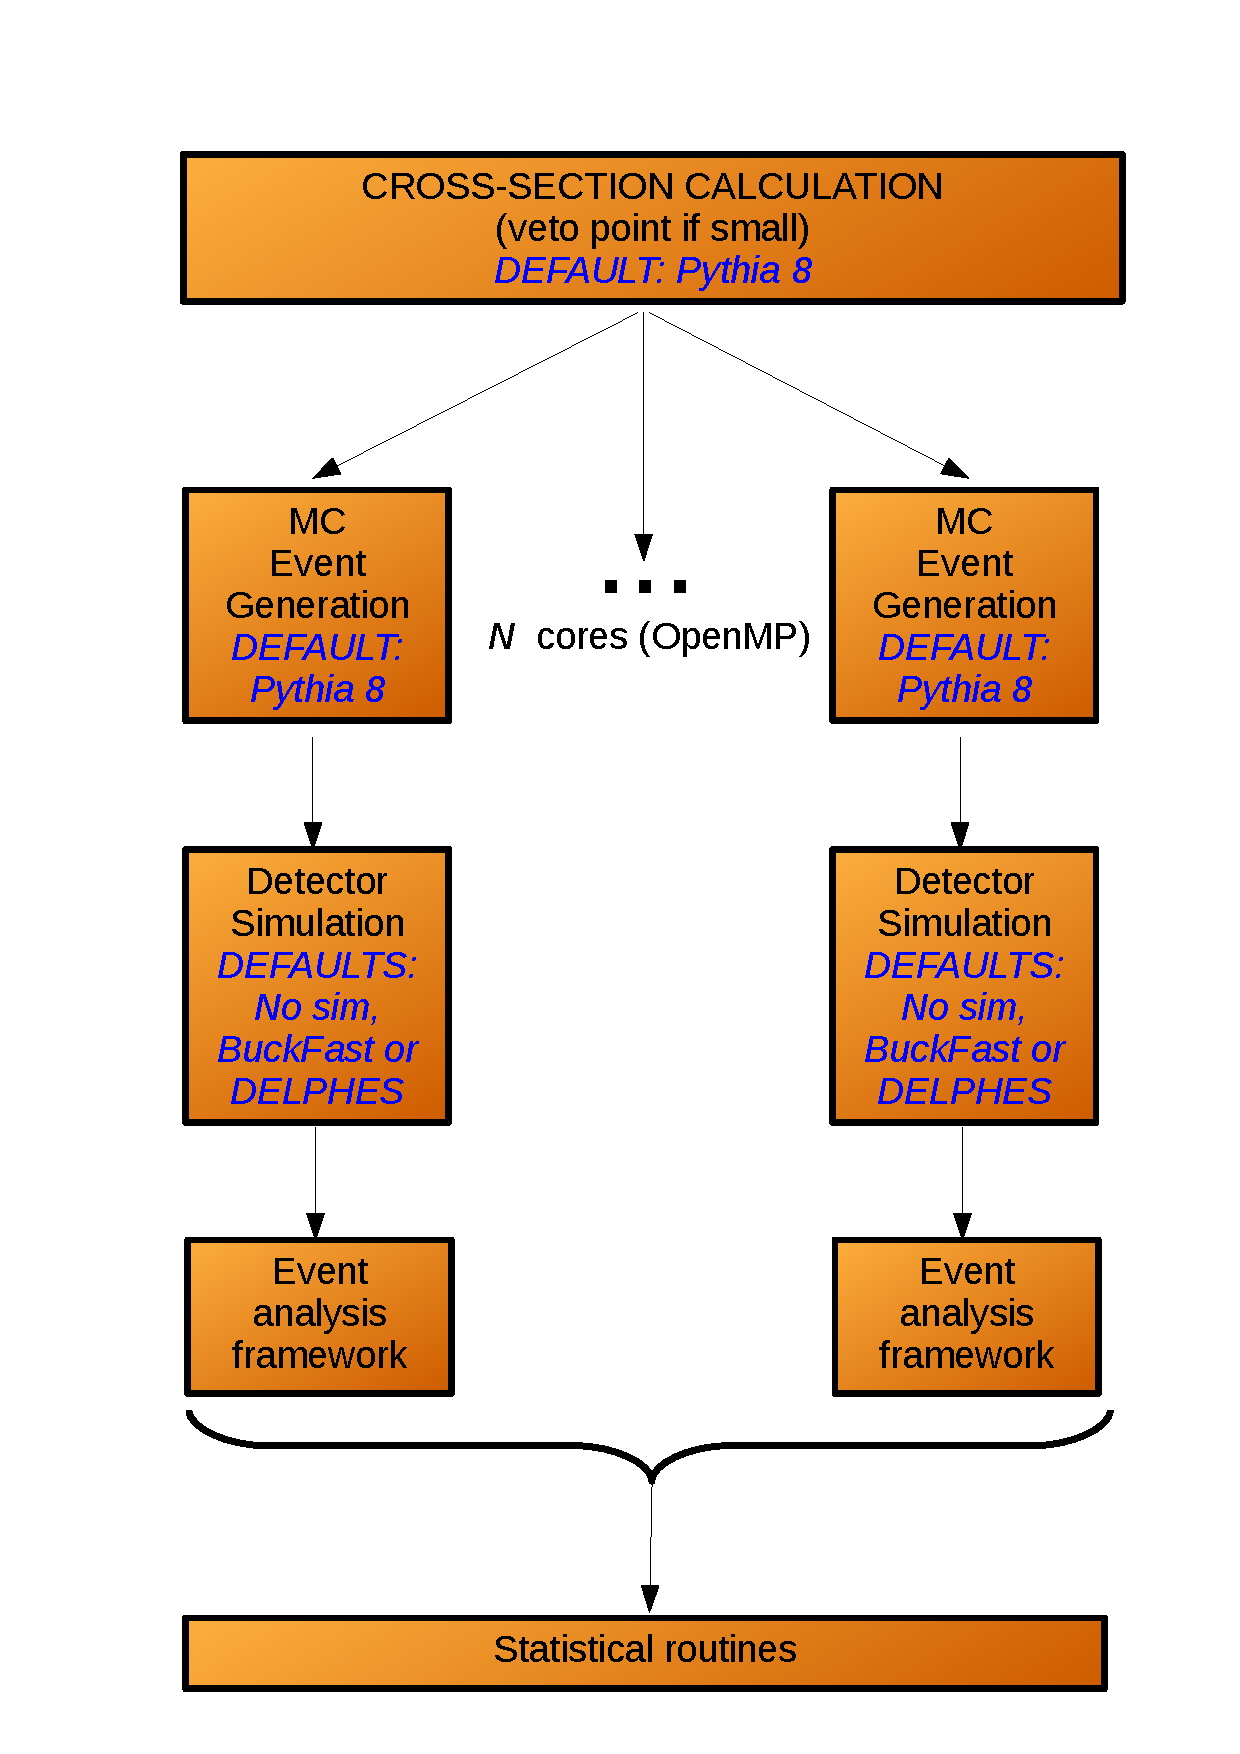
\includegraphics[width=0.8\textwidth]{figures/Gambit-LHC-Chain.pdf}
\caption{Schematic diagram of the \tt ColliderBit \rm processing chain for LHC likelihoods.\label{fig:lhcchain}}
\end{figure}

\subsubsection{Cross-section calculations}

We use the LO+LL cross-sections calculated numerically by the popular \tt Pythia 8 \rm event generator. For many models, these are state of the art. For models where a NLO (or better) calculation is available (e.g. SUSY) our results are conservative, but considerably quicker to evaluate than the full NLO results obtained using the standard \tt Prospino \rm tool~\cite{Beenakker:1996ed}. 

\textbf{For the first release, we should also provide an easy method of having a user-supplied cross-section, perhaps by adding a module function that reads the cross-section from a text file.}

\subsubsection{Monte Carlo event generation}

We supply an interface to the \tt Pythia 8 \rm event generator, alongside custom code that parallelises the main event loop of \tt Pythia \rm using \tt OpenMP \rm (for a similar approach, see~\cite{Lester:2005je}). This allows generation of $\approx$ 10,000 SUSY events on an Intel Core i7 processor in less than 10s (\textbf{Should we note the necessary compile options here?}). In addition, in a GAMBIT-driven global fit, points are vetoed if the production cross-section is already too low to lead to observable consequences at the LHC, giving an implicit speed increase. Taken together, these routines make the running of a full Monte Carlo simulation in a global fit computationally tractable. The choice of the \tt Pythia \rm generator is an acceptable compromise between generality and ease of use for the first \tt ColliderBit \rm release. It is sufficient for many BSM models, and is easily extendable with matrix elements for new models via the existing \tt Madgraph 5 \rm interface (for an example, see Section ADD). \tt Pythia \rm will prove insufficient, however.  where NLO diagrams are significant (for example, in the accurate treatment of some effective field theories of dark matter in LHC monojet searches, where top quark loops become important~\cite{Buckley:2014fba}). These deficiencies can be fixed in the current release via a user-supplied interface to an appropriate Monte Carlo tool, and such interfaces will be supplied as standard in future \tt ColliderBit \rm releases.

\textbf{Should we provide instructions for how to interface to a new MC tool for the first release? Perhaps we should to make sure that ColliderBit doesn't fall over.}

\subsubsection{Detector simulation}
\tt ColliderBit \rm is structured so that the detector simulation is run during the parallelised main event loop, thus giving an implicit speed increase of the simulation step. The user has several options for this step, and in all cases jets are reconstructed usiung the \tt Fastjet \rm package~\cite{Cacciari:2011ma}.

\begin{center}
\emph{No detector simulation}\\
\end{center}

The user can choose to run no detector simulation, in which case the truth level MC events are passed directly to the event analysis framework. Jets may be defined directly at the parton level, or at the hadron level. The former is only really sufficient for analyses in which leptons are the main species of interest, in which case turning off hadronisation can lead to a large speed increase.

\begin{center}
\emph{Delphes}\\
\end{center}

We provide an interface to the \tt DELPHES \rm detector simulation (\textbf{Which version?})~\cite{deFavereau:2013fsa,Ovyn:2009tx} which provides respected simulations of the ATLAS and CMS detectors. DELPHES includes a simulation of track propagation in the magnetic field of an LHC detector, along with a simulation of the electron and hadron calorimeters, and the muon chambers. The user can configure the parameters of the simulation using the normal DELPHES card, but it should be noted that $b$ tagging and the ATLAS lepton ID selection efficiencies (``medium'',''tight''), etc, are applied within the event analysis framework in order to allow different analyses to use different working points.

\begin{center}
\emph{BuckFast}\\
\end{center}

For many purposes, a more approximate (and much faster) approach based on four vector smearing is sufficient, and we therefore also supply an internal \tt ColliderBit \rm detector simulation, \tt BuckFast \rm, that uses a mixture of the DELPHES momentum and energy resolution functions and new parameterisations of the ATLAS and CMS identification efficiencies, as follows: (\textbf{Need to add CMS functions for first release. Also should we update the DELPHES functions used for the initial efficiency and resolution?}.  

\begin{itemize}
\item \textbf{Electrons: }We apply, to the truth level electron four vectors, the DELPHES functions for electron tracking efficiency, electron energy resolution and electron reconstruction efficiency (in that order). In the analysis step, we apply parameterisations of the ATLAS medium and tight identification efficiencies (as appropriate), taken from~\cite{ATLAS-CONF-2014-032}.
\item \textbf{Muons: }We apply, to the truth level muon four vectors, the DELPHES functions for the muon tracking efficiency, the muon momentum resolution and the muon reconstruction efficiency (in that order). 
\item \textbf{Taus: }Hadronic taus are identified at truth level, and selected using a flat 40\% efficiency. The energy is smeared by a 3\% jet energy resolution.
\item \textbf{Jets: }Jets are reconstructed at hadron level using the anti-kT algorithm of the \tt Fastjet \rm package \textbf{Need to add configurable jet radius.} The energy is smeared by a 3\% jet energy resolution.
\item \textbf{Missing energy: }\textbf{Andy? I can't remember exactly how we do this.}
\end{itemize}

Andy to add a selection of DELPHES vs BuckFast validation plots for a representative signal process. Should also add some cutflow comparisons (MJW)?

\subsubsection{Event analysis framework}

\begin{itemize}
\item Describe event analysis framework
\item Emphasise applicability to simulated and/or reconstructed events
\item Describe the LHC analyses included in the module and include some validation plots showing some nicely reproduced ATLAS and CMS limits.
\item Explain how to add new analyses
\end{itemize}

\subsubsection{Statistics}
\label{sec:stats}
\begin{itemize}
\item \textbf{Pat to describe the likelihoods implemented in ColliderBit.cpp (i.e. quote formulae for log normal and Gaussian error distributions).}
\end{itemize}
Having obtained a likelihood for each CMS and ATLAS signal region, we calculate the overall LHC likelihood by using the observed likelihood obtained using the signal region that gives the best expected limit. This is conservative, but is the appropriate treatment when one lacks sufficient information to handle correlated systematic uncertainties.

\subsection{LEP likelihood calculation}
\textbf{Are to write short summary.}

\subsection{Higgs likelihood calculation}
\textbf{Chris Rogan to write short summary.}


\section{Examples}
\label{sec:examples}
\textbf{Give some tutorial-style examples for common use cases.}


\subsection{MSSM example}

\begin{itemize}
\item \textbf{Reproduction of an LHC CMSSM exclusion limit?}
\item \textbf{How to scan over pMSSM parameters and return a likelihood.}

\end{itemize}


\subsection{Generic Pythia model example}
Give an example of Madgraph matrix element code to Pythia 8, show how to get it working and how to scan over the parameters and return a likelihood. Might be ambitious for the first paper, but it wouldn't take too long and would be a superb feature for increasing the user base.


\section{Conclusions}

\section{Acknowledgements}

\section{Appendix: Validation (optional)}

\bibliography{biblio}
\bibliographystyle{unsrt}


\end{document}
